%Tipo de documento
\documentclass[12pt,a4paper]{article}

\usepackage[backend=biber,style=apa,citestyle=apa]{biblatex}
\addbibresource{mendeleybib/tesis.bib}

%Idioma y caracteres del idioma
\usepackage[utf8]{inputenc}
\usepackage[spanish]{babel}

%Opción para incluir gráficos
\usepackage{graphicx}
\usepackage{float}
\usepackage{caption}
\usepackage{subcaption}	
\usepackage{enumitem}
\usepackage{stix}        %para el elerdendots para el rango


\usepackage{datetime}	%fecha
\usepackage{mfirstuc}	%mayuscula


%Opciones para incluir caracteres matemáticos
\usepackage{amsmath}
\usepackage{amsfonts}
\usepackage{amssymb}

\usepackage{listings} %codigos de programas

%Opciones de márgenes
\usepackage[left=3cm,right=3cm,top=2.5cm,bottom=2.5cm]{geometry}

\newdateformat{monthyeardate}{%
\monthname[\THEMONTH ] \THEYEAR}

\usepackage{makeidx}
\usepackage{subfiles}
\usepackage[table,x11names]{xcolor}


\newcommand{\tarea}[1]{
{\huge\color{red}{#1}}
}


\newcommand{\tarealista}[1]{
{\Large\color{blue}{#1}}
}


\newcommand{\duda}[1]{
{\Large\color{yellow}{#1}}
}



\makeindex


\begin{document}


%Todo esto es la portada - >



\begin{titlepage}

\begin{center}
\begin{figure}[htb]
\begin{center}

\includegraphics[scale=0.7]{imagenes/logo_u.png}			%hubicaion del logo de la u
\end{center}
\end{figure}

\vspace*{2cm}

UNIVERSIDAD ANDRÉS BELLO

FACULTAD DE INGENIERÍA

INGENIERÍA CIVIL INDUSTRIAL
\&
INGENIERÍA EN AUTOMATIZACIÓN Y ROBÓTICA

\vspace*{2.5cm}

\begin{huge}
\textbf{Control por minimización de recursos en invernadero modular}
\end{huge}

\vspace*{2.5cm}
Alumno:

Hans Christopher Raddatz Garcia

\vspace*{0.5cm}
Profesores guía:
\vspace*{0.5cm}

Samantha Camila Reid Calderón



Nestor M. Palominos Gonzalez

\vspace*{2cm}

\begin{flushright}

TRABAJO DE TESIS PRESENTADO EN CONFORMIDAD 

A LOS REQUISITOS PARA OBTENER EL GRADO DE 

INGENIERO CIVIL INDUSTRIAL E

INGENIERO EN AUTOMATIZACIÓN Y ROBÓTICA

\end{flushright}

\vspace{2cm}

SANTIAGO - CHILE

2020

\end{center}

\end{titlepage} % <- Hasta acá termina la portada

%Pagina de declaración que hiciste las cosas tú

\pagebreak

\begin{center}
\begin{figure}[htb]
\begin{center}

\includegraphics[scale=0.7]{imagenes/logo_u.png}
\end{center}
\end{figure}

\vspace*{2cm}

FACULTAD DE INGENIERÍA \vspace*{0.5cm}

INGENIERÍA CIVIL INDUSTRIAL \vspace*{0.5cm}

INGENIERÍA EN AUTOMATIZACIÓN Y ROBÓTICA \vspace*{0.5cm}

DECLARACIÓN DE ORIGINALIDAD Y PROPIEDAD

\end{center}

\vspace*{3cm}

Yo, Hans Christopher Raddatz Garcia, declaro que este documento no incorpora material de otros autores sin identificar debidamente la fuente. 

\vspace*{4cm}

\begin{flushright}
Santiago, \monthyeardate\today

\vspace{2cm}

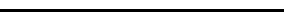
\includegraphics[scale=1]{imagenes/linea.png} 

Firma del alumno

\end{flushright}

\pagebreak		% <----- Término de declaración

%Aquí se pone una frase inspiradora

\vspace*{20cm}

\begin{flushright}

\textit{``Allahu Akbar''}

\end{flushright}

\pagebreak % <--------- Término de frase inspiradora

% Agradecimientos a la vida


\begin{large}

\textbf{Agradecimientos}



\end{large}

\vspace*{1cm}

A mi negro el lucho y al ramundo por ayudarme a obtener la materia para esta Tea-sis.


A la Sami por corregirme esto cuando se veía mas feo.


A mi papá por tenerme la paciencia para armar ``los palos''.


A la pelusa por venir a maullar a mi ventana cuando escriba esto.


Y a cualquiera que sienta que deba estar acá.

\pagebreak			% <-------- Fin te página de agradecimientos

\tableofcontents	% <--------- Se genera la tabla de contenidos, solita!!!

\pagebreak

\listoftables		 % <--------- Se genera la tabla de tablas, solita!!!

\pagebreak

\listoffigures		% <--------- Se genera la tabla de figuras, solita!!!

\pagebreak









\printindex










\section{CONTEXTO}

En la actualidad, la población mundial funciona bajo una serie de recursos de distintos tipos como hídricos, eléctricos, alimenticios, entre otros, los cuales son limitados y necesarios para el funcionamiento colectivo \parencite{FAO2018}. La mayoría de estos recursos presenta problemas, debido a que se están agotando a un ritmo acelerado, por lo que es imperioso proponer medidas o establecer metodologías que permitan un consumo eficiente. 

Los recursos hídricos representan un problema actual, especialmente con su uso en la agricultura \parencite{Specht2014}. En la Figura \ref{fig:agua_dulce_sector} se contempla el porcentaje de agua dulce extraída para los sectores domésticos, industriales y agrícolas, en distintos continentes, donde la mayoría se orienta a esta última área. Además, cabe mencionar que esta área el uso de las tecnologías y técnicas prioriza más la cantidad que la eficiencia. Un ejemplo es la utilización de \textit{Sprinklers} o aspersores de riego por sobre los sistemas de Riego por Goteo Subterráneo (SDI), a pesar que este último presenta ahorros entre el 20\% y el 30\% \parencite{Zaccaria2017}.

   		 
\begin{figure}[h!]
  \centering
    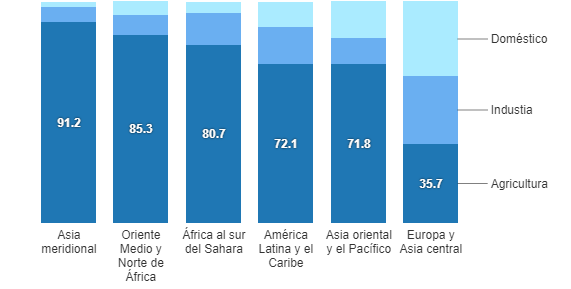
\includegraphics[scale=1]{imagenes/agua_dulce_sector.png}
  \caption{Porcentaje de extracción de agua dulce por sector en 2014. Fuente: (Banco Mundial 2017)}
  \label{fig:agua_dulce_sector}
\end{figure}   	

De igual manera, el consumo del recurso energético (específicamente el eléctrico) ha ido incrementando a nivel global, como se indica en la Figura \ref{fig:PRIMEC}. Sin embargo, su costo ha ido disminuyendo, lo cual ha incentivado su uso (especialmente en la agricultura), como se muestra en la Figura \ref{fig:ENEINTEC}.

  		\begin{figure}[H]
  		\centering
    	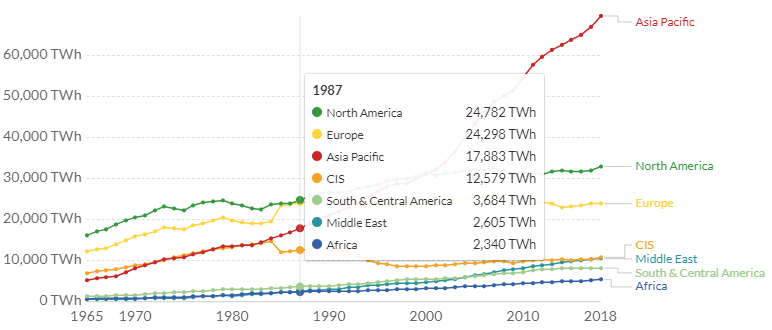
\includegraphics[width=\linewidth]{imagenes/Primary energy comsumption by worl region(BP Stadistical Review of World Enegy(2019)).PNG}
  		\caption{Registro histórico del consumo eléctrico según continentes. Fuente: (BP , 2019)}
  		\label{fig:PRIMEC}
		\end{figure}%
		
			
		\begin{figure}[H]
  		\centering
   		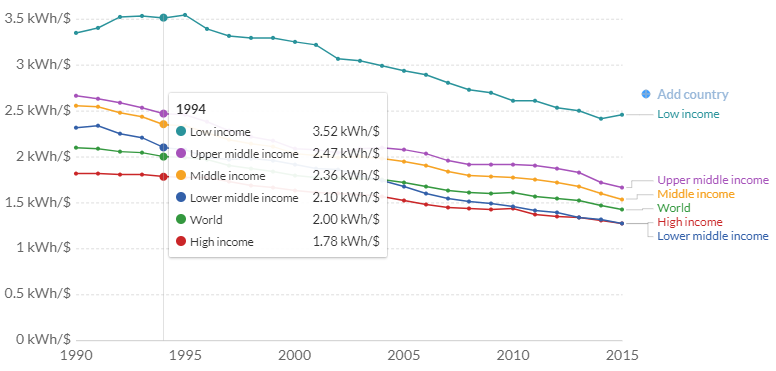
\includegraphics[width=\linewidth]{imagenes/Energy intensity of economics(World Bank, Sustainable for All).PNG}
  		\caption{Precio promedio mundial de la electricidad. Fuente: (World Bank,2016)}
  		\label{fig:ENEINTEC}
  		\end{figure}

Por otro lado, el consumo de alimentos ha ido incrementando, principalmente debido a un aumento en la población. Según la FAO (2018), se espera que se consuma el doble para el año 2015. Su demanda histórica se visualiza en la Figura \ref{fig:FAOFOOD}, donde se muestra el consumo de alimentos para personas, ganado y otros usos.

\begin{figure}[h!]
  \centering
    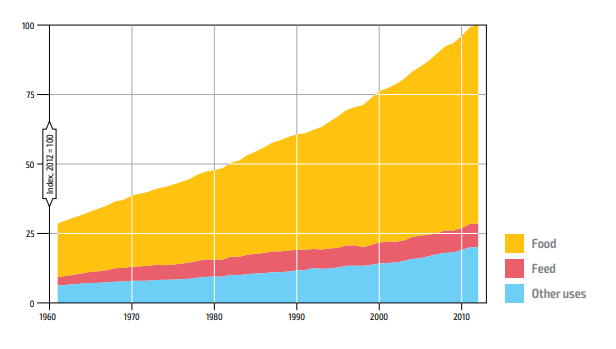
\includegraphics[scale=0.7]{imagenes/Food and non-food agricultural demand historical trends cut.png}
  \caption{Demanda historica en la agricultura. Fuente: \parencite{FAO2018}}
  \label{fig:FAOFOOD}
\end{figure}

Finalmente, con todos estos recursos limitados, es necesario confeccionar metodologías para promover un mejor uso en el área de la agricultura, como lo es el uso de invernaderos.

\subsection{Invernaderos}
\tarea{agregar ejemplos con fotos}
	Los invernaderos son herramientas que permiten disminuir el  consumo hídrico y la necesidad de condiciones medio ambientales específicas, haciendo uso de otros recursos, como la electricidad o gas natural. Asimismo, presenta la capacidad de controlar y a su vez monitorear ciertas variables, tales como la temperatura, humedad e iluminación entre otros \parencite{Specht2014}. Estos suelen construirse de tal forma que mejoren de forma pasiva el entorno en que los cultivos son plantados, logrando así aislarlos de los cambios de temperatura, lluvia y los fuertes vientos. Estos invernaderos pueden tener muchas formas de construcción, pero tienden a seguir un ``estándar`` en lo que respecta a tamaño, irrigación, calefacción e iluminación, siendo estos de un considerable tamaño para albergar la mayor cantidad de plantas en él. 

	La utilización de irrigación por aspersores o aspersorios en los invernaderos son los mismos que se utilizan en los cultivos a la intemperie. La temperatura del aire atrapado dentro del invernadero puede ser controlado variando el uso de tuberías de calefacción o ventanas al exterior. Por último la iluminación se logra mediante un ``techo`` que permita el paso de la luz solar como fuente de iluminación \parencite{Specht2014}.
	
	
%	\paragraph{}	
%	Para la construcción del invernadero se considera la utilización de las siguientes tecnologías:
%	\begin{itemize}
%		\item SDI(subsurface drip irrigation) el cual funciona mediante goteo del agua al nivel de la raíz y que a demostrado ser al menos un 20\% más eficiente que los Sprinklers(aspersores) \parencite{Zaccaria2017}
%		\item Iluminación asistida, la cual ha probado ser de gran potencial para las zonas o lugares con escasa luz solar \parencite{Darko2014}.
%		\item Calefacción del subsuelo, tecnológica que se ha utilizado principalmente en conjunto a paneles solares para calefaccionar el agua con el fin de almacenarla y entregarla a través del suelo por debajo de los cultivos \parencite{Cuce2016}.
%	\end{itemize}
	
%Nota8: Hablar brevemente de los distintos tipos de invernaderos. Por ejemplo, partir por el modelo clásico yl uego el modular con el que vas a trabajar tu.

\section{IMPORTANCIA DEL TRABAJO}


Como se mencionó anteriormente, el sector agrícola es un área poco desarrollada en cuanto al uso eficiente de recursos, siendo una de las actividades que más afecta el consumo de agua a nivel global. Esto se ve reflejado en distintos elementos, tal como es el caso de la irrigación, donde aún se ocupan elementos como los Sprinklers. 

Otra importancia radica en la creciente necesidad de alimentos debido al aumento de población, mientras existe una disminución en las áreas de suelo arable. Debido a esto, se genera una necesidad de habilitar nuevos espacios para la actividad o utilizar tecnologías que permitan un uso mas eficiente del suelo o de suelos antes no disponibles. Un ejemplo de esto son los invernaderos verticales, los cuales permiten multiplicar la producción por metro cuadrado \parencite{Specht2014}. Sin embargo, la metodología de construcción de este tipo de invernadero con tecnologías altamente eficientes es escasas.			
\section{DISCUSIÓN BIBLIOGRÁFICA}

	Un invernadero automatizado requiere de un control preciso y oportuno para la minimización del consumo de los recursos utilizados. Varios autores abordan la problemática del control de los invernaderos en diversas áreas como lo son la iluminación, irrigación y calefacción entre otras. Algunos autores como \textcite{Hasni2011, Singhal2017, Chen2018} utilizan para su modelación el uso de heurísticas para un control más rápido y/o preciso.
	
\subsection{Marco teórico de modelos de gestión de recursos}

	
	
	 A continuación, se explica las aproximaciones que tomaron los autores mencionados en el cuadro \ref{tab:modelos} y \ref{tab:contru} para los controles de la calefacción, irrigación e iluminación. 
	 
		La irrigación en la agricultura suele realizarse mediante Sprinklers (aspersores), por ello autores como \parencite{Gijzen1998, Dong2018} modelan los invernaderos considerando el uso de esta tecnología como método de irrigación. A pesar de ser los métodos más utilizados, autores como \parencite{Of2000, Kazumba2010, Zaccaria2017} han demostrado de forma experimental que el uso de SDI (irrigación en el subsuelo) llegan a ser más eficiente en el uso de agua que los Sprinklers. Dentro de los autores del cuadro \ref{tab:modelos}, el autor \parencite{Kandelous2010} es de los pocos que modelan el sistema SDI, el cual tiene la complejidad de tener que calcular el desplazamiento por capilaridad y gravedad a través del suelo pero, a diferencia del uso de Sprinkler, no es necesario calcular pérdidas de evaporación.
		
		Por otra parte, la calefacción para invernaderos es el tópico más abordado por los autores del cuadro \ref{tab:modelos}, ya que se considera como uno de los mayores consumos dentro de un invernadero\parencite{Chen2015}. Debido a la alta complejidad matemática del sistema producida por la dinámica de fluidos, ciertos autores utilizan modelos heurísticos, principalmente la optimización de enjambre de partículas (PSO) \parencite{Hasni2011,Chen2018}, el cual simplifica la dinámica de la temperatura del aire atrapado dentro del invernadero. El autor\parencite{Singhal2017} utiliza algo parecido, pero con el uso de optimización de lobo gris (GWO), con el cual logró mejores resultados en dicho trabajo por la naturaleza de la termodinámica(convección). Otros autores como \textcite{Kurpaska2000}, modeló un sistema donde se elevó la temperatura del suelo y en consecuencia, aumentó la del aire. En dicho trabajo se contrastaron ambos sistemas, logrando mejores eficiencias en los intercambiadores enterrados. Ambos sistemas pueden ser visualizados en la figura \ref{fig:heat}.

		\begin{figure}[h!]
  			\centering
    		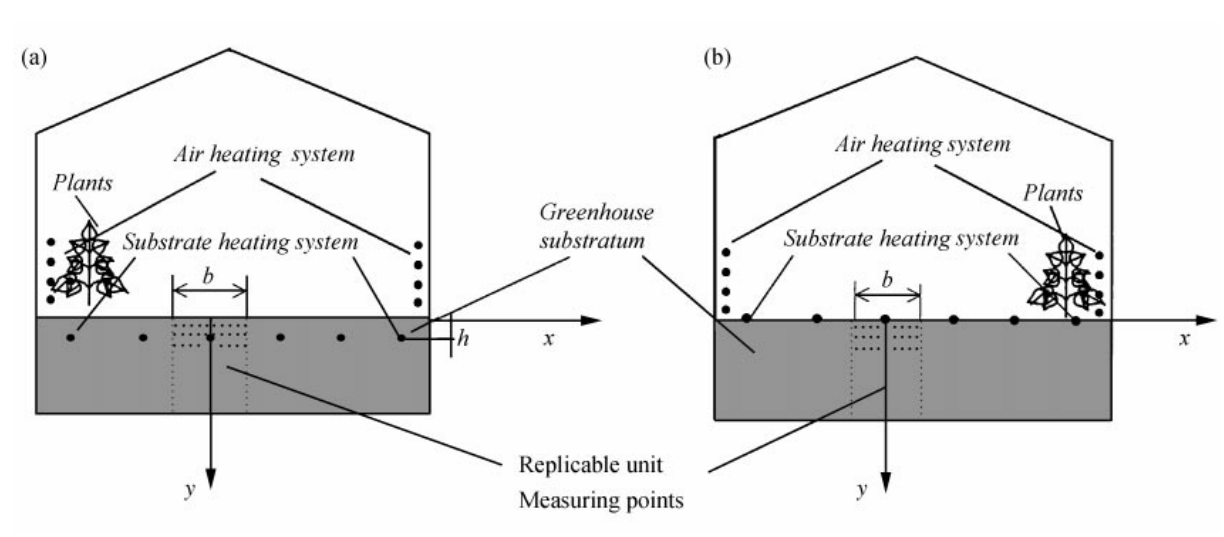
\includegraphics[width=\textwidth]{imagenes/heat_pipe.PNG} 
  			\caption{a) Sistema convencional   b) Sistema subsuelo. Fuente:  \parencite{Kurpaska2000}}
  			\label{fig:heat}
		\end{figure}
			
		En cuanto a iluminación, debido a que la mayoría de los invernaderos estudiados son de tipo ''venlo'' (estructuras transparentes de vidrio o plástico) la iluminación no es una variable que se pueda controlar, ya que esta proviene de la luz solar y es atenuada por el material de construcción. Debido a que su efecto no perdura en el tiempo, esta es una variable en que su control esta meramente determinado por la iluminación del sol. Según \parencite{Darko2014} cada planta tiene un rango en el nivel de luz en donde la fotosíntesis es más efectiva y por ello \parencite{VanIersel2017} aborda el control de esta variable graduando un pulso modulado(PWM), para el cual se hizo una regresión lineal respecto a los valores entregados por una tira LED(diodo emisor de luz) al respectivo valor del PWM.
		\newpage
		
\subsection{Marco teórico de modelos de optimización en la gestión de recursos en un invernadero}	
		

A continuación, se muestra una pequeña descripción del trabajo de cada autor de la tabla \ref{tab:modelos}.
	
	{
	\paragraph{\cite{Kurpaska2000}}	 desarrolla un modelo que minimiza la temperatura del líquido que fluye dentro de los intercambiadores de calor en un invernadero, además de responder a que distancia de las superficie del suelo se deben colocar los intercambiadores en el subsuelo.
		
	\paragraph{\cite{Kandelous2010}} desarrolla un modelo para minimizar el uso de agua en sistemas de irrigación SDI para luego compararlo con el modelo numérico HYDRU-2D, el software analítico WetUp, y otros modelos empíricos por el mismo autor en 2008.
		
	\paragraph{\cite{Hasni2011}} desarrolla un modelo de PSA (algoritmos de enjambre de partículas) y AG (algoritmo genético) para minimizar el costo operacional de la calefacción. Considerando que la tierra se calienta y aire encerrado en el invernadero. 


	\paragraph{\cite{Kiyan2013}} desarrolla un modelo de calefacción con fuente híbrida (solar/fósil) para minimizar el consumo de combustible en función del entorno (temperatura e iluminación) y los parámetros propios del invernadero.
		
		
	\paragraph{\cite{Bozchalui2015}}desarrolla un modelo para minimizar los costos operacionales de iluminación y producción de CO2 según una predicción del clima, además se introduce el efecto de las ``Smart-Grid'' en la variación de precios para la electricidad. Las variaciones es estas predicciones son estudiadas a través de la simulación de montecarlo.


	\paragraph{\cite{Chen2015}} Desarrolla un modelo utilizando CDF (dinámica de fluidos computacional) más un modelo de predicción para minimizar únicamente los costos operacionales de la calefacción en invernaderos.

		
	\paragraph{\cite{Singhal2017}} desarrolla un modelo para el control de la calefacción mediante el uso de GWO (optimización del lobo gris), luego compara sus resultados con otras técnicas como PSO y AG.


		
	\paragraph{\cite{Chen2018}} desarrolla un modelo robusto para el control de la temperatura a través de MPC (modelo predictivo de control), para ello utiliza PSO que permite incluir una posible perturbación, la cual suele ser omitida por otros autores. Comparó el MPC con y sin PSO vinculándole un ruido sinusoidal.
	
	
	\paragraph{\cite{Dong2018}} Utilizando partes de los modelos en \cite{Gijzen1998} desarolla un modelo centrado en un invernadero de una cara para la minimización de los costos de calefacción según las condiciones externas
	}	
		
		\paragraph{}	%tecnologias modelados, 		
		A continuación, se muestran dos tablas de los autores relevantes para este trabajo. En ellas se ordenan los autores respecto al tipo de contribución (construcción o modelado), a su vez, se muestra las variables que se trabajan en dichos documentos. También, se distinguió si el control que realizo para dicha(s) variable(s) fue realizada como: una predicción del comportamiento en el tiempo, un control en tiempo real o si no efectuó control alguno. Finalmente, se muestra si es que el autor realizó una aplicación experimental o no.
	




% Please add the following required packages to your document preamble:
% \usepackage{graphicx}
\begin{table}[h!]
\centering
\caption{Marco teórico de construcción de un invernadero}
\label{tab:contru}
\resizebox{\textwidth}{!}{%
\begin{tabular}{|l|l|l|c|l|l|c|c|}
\hline
Autor       & Año  & Objetivo                                         & 1 & 2 & 3 & Tipo de control & Experimental \\ \hline
E. Suarez   & 2000 & Comparación de tipos de irrigación Sprinkler/SDI & X &   &   & R               & X            \\ \hline
Kazumba, S. & 2010 & Uso de SDI con agua recuperada                   & X &   &   & R               & X            \\ \hline
F. R. Lamm  & 2010 & Estado de la tecnologia SDI                      & X &   &   & N               &              \\ \hline
Xiaoning M. & 2012 & Analizar patrones por el riego mediante SDI      & X &   &   & N               & X            \\ \hline
Cuce E.     & 2016 & Analizar métodos  sostenibles para invernaderos  &   & X & X & N               &              \\ \hline
Marc W.     & 2016 & Proponer una metodologia de iluminacion asistida &   &   & X & R               & X            \\ \hline
\rowcolor{yellow}Propuesta	& 2020 & Desarrollo de un invernadero modular eficiente   & X & X & X & P
& X			   \\ \hline
\end{tabular}%
}

\end{table}






\begin{table}[h!]
\centering
\caption{Marco teórico de modelos de optimización en la gestión de recursos}
\label{tab:modelos}
\resizebox{\textwidth}{!}{%
\begin{tabular}{|l|l|l|c|l|l|c|c|}
\hline
Autor        & Año  & Función Objetivo                                                    & 1 & 2 & 3 & Tipo de control & Experimental \\ \hline
%Gijzen, H.   & 1998 & Simular cultivos dentro de un invernadero                           & X & X &   & N               &              \\ \hline
Kurpaska, S. & 2000 & Minimizar altura de tubos de calefacciónado subterraneos            &   & X &   & P               & X            \\ \hline
Kandelous, M & 2010 & Minimizar el uso de agua para regadío & X &   &   & P               & X            \\ \hline
Hasni, A.    & 2011 & Minimizar gasto en calefacción mediante heurística                  &   & X &   & P               & X            \\ \hline
Kiyan, M.    & 2013 & Minimizar temperatura requerida para calefaccionar un invernadero                          &   & X &   & R               & X            \\ \hline
Mohammad, C. & 2015 & Minimizar gasto en calefacción e iluminación en "Smart Grids"       &   & X &   & P               &              \\ \hline
Chen, J.     & 2015 & Minimizar costos operacionales de Calefacción                                  &   & X &   & P               & X            \\ \hline
Singhal, R.  & 2017 & Minimizar gasto en calefacción mediante heurística                  &   & X &   & P               &              \\ \hline
lijun, C.    & 2018 & Minimizar gasto en calefacción mediante heurística                  &   & X &   & P               &              \\ \hline
Shuyao D.    & 2018 & Minimizar consumo eléctrico en invernaderos                                      &   & X &   & N               & X            \\ \hline
\rowcolor{yellow} Propuesta	 & 2020 & Minimizar costos operacionales de un  invernadero modular 		  & X & X & X & X			    & X			   \\ \hline
\end{tabular}%
}
\end{table}



\begin{table}[h!]
\centering
\resizebox{\textwidth}{!}{%
\begin{tabular}{llll}
\hline
(1) = irrigación            & (2) = temperatura       & (3) = Iluminación & R = Control en tiempo real                             \\ \hline
 P = Control predictivo & N = Sin control  & X = Realiza un experimento & \\ \hline
\end{tabular}%
}
\end{table}


		

		
		
		
	
		

\section{CONTRIBUCIÓN DEL TRABAJO}
	La contribución del trabajo se divide en: (a) diseñar y confeccionar un sistema para invernaderos modulares que permita la comunicación, control y visualización de  múltiples "módulos" de invernaderos automatizados; y (b) desarrollar un modelo de optimización que minimice los costos por el uso del sistema de irrigación y temperatura en el tiempo.
	
\section{HIPÓTESIS}

Un invernadero automatizado que realice un control mediante un modelo matemático sera más eficiente que un control realizado por métodos más convencionales.

\section{OBJETIVO GENERAL}

Desarrollar un sistema de gestión para la automatización de invernaderos modulares, minimizando costos operacionales.

\section{OBJETIVOS ESPECÍFICOS}
	\begin{itemize}
    	\item   Confeccionar una maqueta/prototipo de un invernadero modular, incorporando sensores de medición (internos y externos) para las variables de temperatura, humedad y luz.
    	\item Confeccionar un sistema de control cerrado para las variables de la irrigación, iluminación y calefacción.
        \item 	Confeccionar un modelo de optimización que minimice los costos por el uso del sistema de irrigación y temperatura en el tiempo.
        \item 	Implementar y obtener resultados del sistema de control y modelo de optimización dentro del invernadero.

	\end{itemize}
	
\section{METODOLOGÍA}
\subfile{contenidos/metodologia2}                    %metodologia en otro archivo
             

\section{RESULTADOS}
	Aun no hay

\section{CONCLUSIONES Y TRABAJOS FUTUROS}
	 darle mas vueltas al modelo.
\section{REFERENCIAS BIBLIOGRÁFICAS}

\printbibliography


\newpage

\subfile{contenidos/anexos}

\end{document}
